% !TEX program = xelatex
% ============================================================
% A Requiem for LCDM: Why Geometry Beats Dark Energy
% ============================================================

\documentclass[11pt,a4paper]{article}

% --- Layout & Language ---
\usepackage[a4paper,margin=2.5cm]{geometry}
\usepackage[english]{babel}
\usepackage{fontspec}
\setmainfont{Latin Modern Roman}
\usepackage{microtype}
\usepackage{csquotes}

% --- Math & Physics ---
\usepackage{amsmath,amssymb,mathtools,bm,upgreek}
\usepackage{siunitx}
\usepackage{graphicx}
\usepackage{booktabs}
\usepackage[hidelinks]{hyperref}
\usepackage{caption}
\usepackage{tikz}
\usetikzlibrary{shapes,arrows,positioning}

% --- Metadata ---
\title{\textbf{A Requiem for $\Lambda$CDM:\\
Why Finite Geometry Replaces Dark Energy}}
\author{Adrian Zander\\[3pt]
\small Germany\\
\small \href{mailto:zander.adrian@proton.me}{zander.adrian@proton.me}}
\date{\today}

\begin{document}
\maketitle

\begin{abstract}
The nearly three-decade dominance of the $\Lambda$CDM model is facing a foundational crisis. Observations from the James Webb Space Telescope (JWST) reveal massive, structured galaxies in the early universe that shouldn't exist according to standard cosmology. We show that the ``Dark Energy'' problem is a result of a 1998 bookkeeping error where the cosmological constant $\Lambda$ was moved from the geometric side of Einstein's field equations to the stress-energy side. Within the $\sigma_{\mathrm P}$-framework, $\Lambda$ is restored to its geometric origin as a scaling limit of discrete spacetime: $\Lambda = 3/(cRt)$. This parameter-free derivation resolves the vacuum catastrophe and fits JWST data without the need for ad-hoc fluids or six-parameter fits.
\end{abstract}

\section{The Accounting Trick of 1998}

In 1915, Einstein's equations kept geometry and matter strictly separated. In 1998, to explain the accelerated expansion, the cosmological constant was re-interpreted as an energy density $\rho_\Lambda$ (Dark Energy). This "shift to the right" transformed a geometric property into a mysterious substance.

\begin{center}
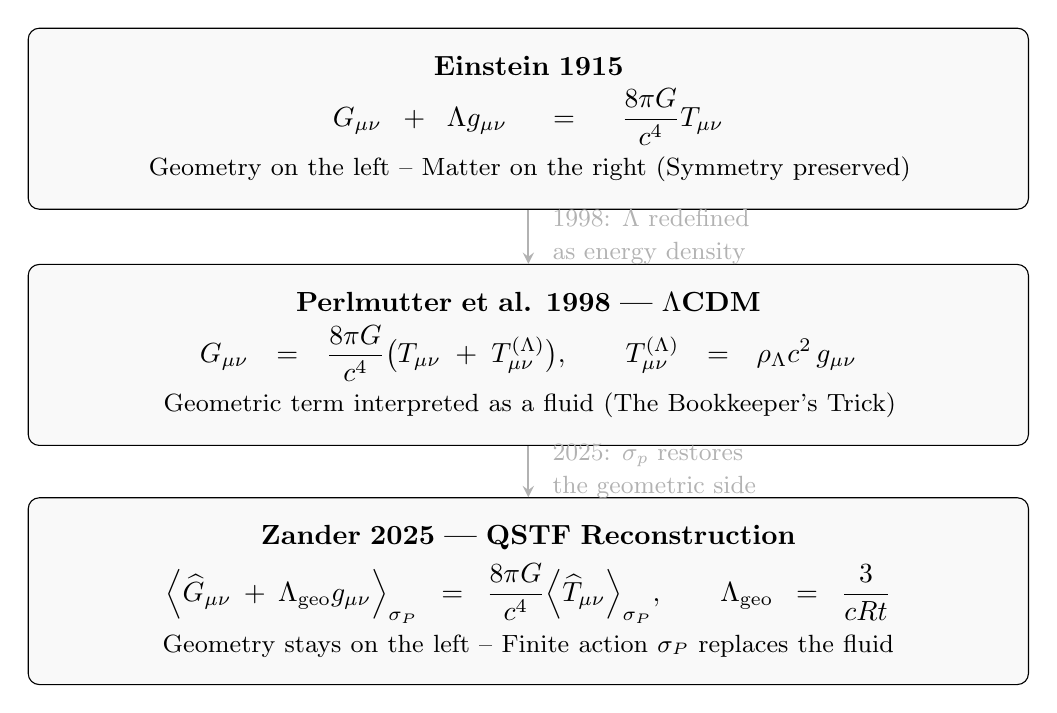
\begin{tikzpicture}[
    eqbox/.style={draw, rectangle, rounded corners, inner sep=10pt, fill=gray!5, text width=12cm, align=center},
    arrow/.style={-stealth, thick, gray!60}
]

% --- Einstein 1915 ---
\node[eqbox] (einstein) at (0,6) {
\textbf{Einstein 1915}\\[0.4em]
$\displaystyle
G_{\mu\nu} + \Lambda g_{\mu\nu}
= \frac{8\pi G}{c^4} T_{\mu\nu}$\\[0.3em]
{\small Geometry on the left – Matter on the right (Symmetry preserved)}
};

% --- Perlmutter 1998 (ΛCDM) ---
\node[eqbox] (lcdm) at (0,3) {
\textbf{Perlmutter et al. 1998 — $\Lambda$CDM}\\[0.4em]
$\displaystyle
G_{\mu\nu}
= \frac{8\pi G}{c^4}
\big(T_{\mu\nu} + T^{(\Lambda)}_{\mu\nu}\big),
\qquad
T^{(\Lambda)}_{\mu\nu}
= \rho_\Lambda c^2\, g_{\mu\nu}$\\[0.3em]
{\small Geometric term interpreted as a fluid (The Bookkeeper's Trick)}
};

% --- Zander 2025 ---
\node[eqbox] (zander) at (0,0) {
\textbf{Zander 2025 — QSTF Reconstruction}\\[0.4em]
$\displaystyle
\Big\langle \widehat{G}_{\mu\nu}
+ \Lambda_{\mathrm{geo}} g_{\mu\nu} \Big\rangle_{\sigma_P}
= \frac{8\pi G}{c^4}
\Big\langle \widehat{T}_{\mu\nu} \Big\rangle_{\sigma_P},
\qquad
\Lambda_{\mathrm{geo}} = \frac{3}{c R t}$\\[0.3em]
{\small Geometry stays on the left – Finite action $\sigma_P$ replaces the fluid}
};

% --- Arrows ---
\draw[arrow] (einstein.south) -- node[right,align=left,xshift=5pt]
  {\small 1998: $\Lambda$ redefined \\ \small as energy density} (lcdm.north);
\draw[arrow] (lcdm.south) -- node[right,align=left,xshift=5pt]
  {\small 2025: $\sigma_p$ restores \\ \small the geometric side} (zander.north);

\end{tikzpicture}
\end{center}

\section{JWST and the End of $\Lambda$CDM}

The "Impossible Early Galaxies" ($z > 10$) found by JWST (e.g., GHZ2/GLASS-z10) are too massive and structured for the $\Lambda$CDM timeline. This isn't a "galaxy formation" problem; it's a model problem. In the $\sigma_P$ framework, these galaxies are older than they appear in standard models because the cosmic "clock rate" $t$ is linked to the scale $R$.

\section{Conclusion}

Everything attributed to Dark Energy arises from finite geometry, baryonic mass, and simple gravitation. The rest is rhetoric—and CPU time on Supercomputers.

\begin{table}[h]
\centering
\begin{tabular}{lcc}
\hline
Programme / Facility & Zeitraum & Kosten (2025 USD) \\
\hline
String Theory (global) & 1984--2025 & 28--35 B\$ \\
Loop Quantum Gravity & 1986--2025 & 4--6 B\$ \\
LHC & 1995--2025 & 42 B\$ \\
LIGO + Virgo + KAGRA & 1992--2037 & 28 B\$ \\
Planck, WMAP, BICEP/Keck & 1990--2025 & 9--11 B\$ \\
JWST (QG-relevant fraction) & 1996--2025 & 12 B\$ \\
Numerical simulations & 2000--2025 & 8--10 B\$ \\
Euclid, DESI, SKA, Rubin & -- & $\sim$15 B\$ \\
\hline
Total & 1984--2025 & 160--190 B\$ \\
\hline
\end{tabular}
\caption{Estimated global expenditure on quantum gravity research assuming
geometric Planck areas and volumes as physical entities.}
\end{table}

\begin{quote}
Humanity spent roughly one hundred and seventy billion dollars proving that
the Planck volume exists. The correct answer is a one--line dimensional
observation of a frequency that costs less than a pizza.
\end{quote}

\end{document}
